\chapter{Background}

\section{The SQL Standard }
DBMS from its first appearance shows that it will be the dominant trend for managing data. Consequently, different implementations have emerged from various vendors and inevitably, a standardised language should be implemented in order to provide portability among current systems. If applications were implemented using only SQL commands which are defined in that standard and vendors implemented these commands in exactly the same way, then SQL code could be migrated on any DBMS without the need to be adopted.

The first appearance of the SQL language was in 1970 where IBM developed the first prototype of Relational Database Management System (RDBMS) [8, 16]. Subsequently, the first SQL standard arose in 1986 by the American National Standard Institute (ANSI) with the name SQL-86 for bearing conformity among vendors’ implementations. Since then, different flavors of the standard have being emerged for revising previous versions or for adding new features such as SQL-87, SQL-89, ANSI/ISO SQL-92 and ANSI/ISO SQL: 1999 which has been approved also by the International Standards Organization (ISO) [2, 11, 21, 22]. The SQL Standard has been continuously developed with current version being SQL:2016 or ISO/IEC 9075:2016. The ANSI SQL standard is divided into several parts and this project focuses on the SQL/Foundation part. This part contains central elements of SQL. Explanations about the findings are explained according to SQL:2016 since it is the newest version of the standard, though this part  remains the same in comparison with earlier flavors. 

\section{The SQL Language}
SQL operations are in the form of commands known as SQL statements. More precisely, SQL is composed of primarily two sublanguages, the data definition language (DDL) and the data manipulation language (DML) [17, 12,23]. DDL is a part of SQL language and can be used to create, modify, delete tables and views, and usually DDL statements start with keywords ‘CREATE’, ‘DROP’ and ‘ALTER’. Also, it supports a command that gives the capability of defining new domains. Moreover, in general, tables and rows are denoted as relations and tuples. DML is also a part of the SQL language that is composed of a family of commands like any programming language and is used for the creation of a query for inserting, modifying and deleting rows in a Database. This sublanguage is consisted by ‘SELECT-FROM-WHERE’ commands as to be the fundamental for any query. In addition, the SQL Standard supports more complex rather than just simple commands for performing various tasks on data. For example, aggregation functions such as ‘Sum’, ‘Max’, ‘Min’, ‘Avg’ are used with combination with ‘Group By’, and ‘Having’ SQL statements. The purpose of having such commands is to perform a calculation on a specific column in order to return a value, for example the calculation of the average salary of a department by performing a ‘Group By’ based on all the salaries of the employees of that department. 

Hence, SQL is extremely popular as it offers two capabilities. Firstly, it can access many tuples using just one command and secondly it does not need to specify how to reach a tuple, for example by using an index or not. 


\section{Commands of SQL}
In this section a high-level description of the basic SQL commands is given, as defined in the Standard. Due to the fact that these commands are used to generate random queries, it is imperative to give a short presentation of each command and its purpose. 

\hfill\newline
\noindent\textbf{\underline{SQL Basic Structure}} 
\begin{mdframed}[nobreak=true, backgroundcolor=lightgray!20] 
\begin{lstlisting}[style=SQL]
SELECT [DISTINCT] columns_list
FROM tables_list
WHERE Condition1 {AND|OR} Condition 2
\end{lstlisting}
\end{mdframed}
 
The SQL basic structure represents the basic SQL commands which are used to retrieve data from a database based on some criterias  that are specified  in the ‘WHERE’ clause. Each SQL query should have at least ‘SELECT’ and ‘FROM’ clause.  The ‘WHERE’ clause is optional. The basic SQL query is executed as followed: all the rows of the tables list in the ‘FROM’ Clause are evaluated. Each row that satisfies the search criteria is selected. Then, only the specified columns of the selected rows appear in the result. In addition,  the ‘DISTINCT’ keyword is optional and can be used to eliminate duplicates rows in the result. Also, instead of having columns\_list in the SELECT clause, the “*” keyword can be used which indicates that all the columns of the tables\_list will appear in the result. The purpose of the ‘WHERE’ clause is to filter the results, normally SQL queries contains a ‘WHERE’ clause. Conditions compare expressions using comparison operators. A comparison operator is used to compare two expressions and logical connectivities, such as AND, NOT and OR are used to connect the conditions.  

\hfill\newline
\noindent\textbf{\underline{Example of basic query:}}
\begin{mdframed}[backgroundcolor=lightgray!20] 
\begin{lstlisting}[style=SQL]
SELECT St.Student_Name
FROM Students AS St 
WHERE St.age >= 20 AND St.age <= 24
\end{lstlisting}
\end{mdframed}

The above example uses the basic SQL structure to build a query. Thus, it retrieves all the Students and based on the criteria of the ‘WHERE’ clause, it returns the name of students who are between 20 and 24 year old. 

\hfill\newline
\noindent\textbf{\underline{SQL Basic aggregation Syntax:}}
\begin{mdframed}[backgroundcolor=lightgray!20] 
\begin{lstlisting}[style=SQL]
SELECT       [DISTINCT]  Columns_list
FROM         Tables_list
WHERE        Condition1 {AND|OR} Condition2
GROUP BY     Columns_list
HAVING       Condition1 {AND|OR} Condition 2
\end{lstlisting}
\end{mdframed}

SQL query with aggregation is used to perform a calculation on specific columns in order to return a value. ‘GROUP BY’ and ‘HAVING’ are used to perform an aggregation. ‘HAVING’ is an optional clause, where aggregation can still be performed using aggregate commands in the ‘SELECT’ clause. A concrete example is given subsequently. 

\hfill\\
\begin{table}[h]
\centering
\caption{Aggregation Commands}
\label{my-label}
\begin{tabular}{|p{2cm}|p{11.5cm}| }
\hline
 \textbf{Operator}  &  \textbf{Use}                                                    \\ \hline
MIN()               & Finds the minimum value of a column                                \\ \hline
COUNT()             & Returns true, if all the comparisons the operator OP return true   \\ \hline
MAX()               & Returns true, if at least one comparison the operator returns true \\ \hline
SUM()               & Returns true, if an element exist in a given set                   \\ \hline
AVG()               & Calculates the average of values of a column                       \\ \hline
\end{tabular}
\end{table}

Aggregate commands can be used both in ‘SELECT’ and ‘HAVING’ clause in combination with the ‘GROUP BY’ clause. The example below illustrates the proper use of aggregation commands.

\hfill\\
\noindent\textbf{\underline{Example:}}
\begin{mdframed}[backgroundcolor=lightgray!20] 
\begin{lstlisting}[style=SQL]
SELECT COUNT(St.student_id), St.Country
FROM Students AS St 
GROUP BY St.Students
HAVING COUNT(St.student_id)  >  3
\end{lstlisting}
\end{mdframed}

The above query makes proper use of the aggregation commands. In particular, it lists the number of students in every country where there are more than three students in this Country.  

\begin{table}[h]
\centering
\caption{Logical  Operators}
\label{my-label}
\begin{tabular}{|p{2cm}|p{11.5cm}| }
\hline
\textbf{Operator} & \textbf{Use}                                                     \\ \hline
EXISTS            & Returns true, if there is at least one row in the subquery         \\ \hline
Op ALL            & Returns true, if all the comparisons the operator OP return true   \\ \hline
Op ANY            & Returns true, if at least one comparison the operator returns true \\ \hline
Op IN             & Returns true, if an element exist in a given set                   \\ \hline
\end{tabular}
\end{table}

\hfill\newpage
\noindent\textbf{\underline{Example:}}
\begin{mdframed}[backgroundcolor=lightgray!20] 
\begin{lstlisting}[style=SQL]
SELECT  *
FROM Students AS St 
WHERE St.Country IN (‘UK’, ‘Netherland’)
\end{lstlisting}
\end{mdframed}
The query above  retrieves all the students who come from UK and Netherland.

\begin{table}[h]
\centering
\caption{SET Commands }
\label{my-label}
\begin{tabular}{|p{3cm}|p{11.5cm}| }
\hline
\textbf{Command}     & \textbf{Use}                                                                                           \\ \hline
UNION {[}ALL{]}     & Returns the combination of the results of two SQL queries                                     \\ \hline
INTERSECT {[}ALL{]} & Return the combination of the results of two SQL queries for rows that,appear in both results \\ \hline
EXCEPT {[}ALL{]}    & Return each row that appear to the first query but does not appear to the second query        \\ \hline
\end{tabular}
\end{table}

By default SET commands remove duplicates in the SQL result. However, we can have duplicates in the result by adding the optional ‘ALL’ keyword for any of the commands above.  

\noindent\textbf{\underline{Example:}}
\begin{mdframed}[backgroundcolor=lightgray!20] 
\begin{lstlisting}[style=SQL]
SELECT Country FROM Students 
UNION
SELECT Country  FROM  Professor
\end{lstlisting}
\end{mdframed}
The above query retrieves the Countries from where there both Students and professors come. 

\begin{table}[h]
\centering
\caption{String Commands}
\label{my-label}
\begin{tabular}{|p{3cm}|p{11.5cm}| }
\hline
\textbf{Operator} & \textbf{Use}                                         \\ \hline
TRIM()            & Returns the string without leading/trailing characters \\ \hline
SUBSTRING()       & Retrieves a subset of the initial string               \\ \hline
CONCAT()          & Concatenate two or more strings                        \\ \hline
REPLACE()         & Replaces a subset of a string with another string      \\ \hline
LIKE              & Returns true, if an attribute matches with a pattern   \\ \hline
\end{tabular}
\end{table}

\hfill\newpage
\noindent\textbf{\underline{Example:}}
\begin{mdframed}[backgroundcolor=lightgray!20] 
\begin{lstlisting}[style=SQL]
SELECT 
SUBSTRING (“SQLSTANDARD”, 1, 3 ) AS SQLExtraction 
\end{lstlisting}
\end{mdframed}

The SQL query above extracts from a string which is given as parameter to the SUBSTRING function the first three characters starting from the position 1. Thus, the results is: \textbf{SQL}

\begin{table}[h]
\centering
\caption{Data Type}
\begin{tabular}{|p{2.5cm}|p{11.5cm}| }
\hline
\textbf{Types} & \textbf{Description}                                                                     \\ \hline
SMALLINT       & Can store a number from a range between -32768 and 32767                                 \\ \hline
INT            & Can store a number from a range between -2147483648 and 2147483647                       \\ \hline
BIGINT         & Can store a number from a range between -9223372036854775808 and 9223372036854775807     \\ \hline
VARCHAR        & Takes as input the length of a variable string which can contains up to 255 characters   \\ \hline
CHAR           & Takes as input the length of a fixed size string which can contains up to 255 characters \\ \hline
\end{tabular}
\end{table}

\textbf{Operator Precedence}

Operator precedence is an important concept for understanding how an SQL query is evaluated and it is also important for determining if major DBMSs follow the same operator precedence. There are cases where the expressions in the WHERE clause are quite complicated and operator precedence defines in which order the expression should be evaluated. The sequence of operators is provided as follows, classified according to their priority, starting from those with the highest priority: 

\begin{itemize}
\item  () 
\item  +, - , ~
\item  *, /, % 
\item  = , \textgreater , \textless , \textgreater= ,  \textless= ,  \textless\textgreater
\item  NOT ,  AND
\item  ALL , ANY , IN , LIKE
\item  = - variable assignment. 
\end{itemize}

Operators that have the same priority are evaluated from left to the right. In addition, parenthesis abrogate the priority of the rest operators and as a result expressions that are enclosed by a parenthesis are evaluated first.    
 
\subsection{Missing values} 
This section aims to provide a basic background regarding null values and present the problems that can be arised from the presence of nulls in a database. In the section of experiments, it is illustrated that many problems can be appeared. SQL uses null marker for missing or unknown values in a database and for that reason null is a reserved word [24]. It is worthy mentioning that null should not be confused with zero value or an empty string. However, Oracle’s database treats the empty string as null[12], and for that reason new issues are arised.  An important consideration is that it cannot be tested if a value of a field is null using usual comparison operators such as  <>, =  and <  but instead IS NOT NULL and IS NULL commands are used. In general, the existence of nulls in a database is the fundamental source of issues and incompatibilities among current DBMS [26, 27]. In addition, for evaluating each comparison with the existence of NULLS a three-valued logic (3VL) is proposed which is an extension of common boolean logic. In boolean logic, an expression can be evaluated only to 2 values such as TRUE AND FALSE, where the negation evaluate to the opposite values. On the contrary with 3VL, in 3VL there is an addition value called unknown and the opposite of it remains the same. In addition, all comparisons involving NULL should be resulted to be unknown according to SQL Standard. Below it is illustrated a truth table for the different comparisons with the suitable outcomes.

\begin{table}[h]
\centering
\caption{Three-Valued logic truth table}
\label{my-label}
\begin{tabular}{|l|l|l|l|l| }
\hline
\textbf{Y} & \textbf{Z} & \textbf{Y OR Z} & \textbf{Y and Z} & \textbf{NOT Y} \\ \hline
True       & True       & True            & True             & False          \\ \hline
True       & False      & True            & False            & False          \\ \hline
True       & Unknown    & True            & Unknown          & False          \\ \hline
False      & True       & True            & False            & True           \\ \hline
False      & False      & False           & False            & True           \\ \hline
False      & Unknown    & Unknown         & False            & True           \\ \hline
Unknown    & True       & True            & Unknown          & Unknown        \\ \hline
Unknown    & False      & Unknown         & False            & Unknown        \\ \hline
Unknown    & Unknown    & Unknown         & Unknown          & Unknown        \\ \hline
\end{tabular}
\end{table}
 
In an SQL query each tuple which is evaluated to true is returned in the result, and tuples that are evaluated to false or unknown are not returned. Comparisons that involving NULLs are considered as False in the WHERE Clause. Hence, If we take into consideration that only Oracle’s db treats empty string as NULL then it can be realized that many problem can be arised. 

\hfill\newline
\textbf{Examples}
\begin{mdframed}[nobreak=true, backgroundcolor=lightgray!20] 
\begin{lstlisting}[style=SQL]
NULL  =  10 is evaluated to Unknown 
\end{lstlisting}
\end{mdframed}

\begin{mdframed}[nobreak=true, backgroundcolor=lightgray!20] 
\begin{lstlisting}[style=SQL]
NULL = NULL is evaluated to Unknown  
\end{lstlisting}
\end{mdframed}

\begin{mdframed}[nobreak=true, backgroundcolor=lightgray!20] 
\begin{lstlisting}[style=SQL]
NULL <= 3  is evaluated to Unknown 
\end{lstlisting}
\end{mdframed}

\hfill\newline 
\begin{mdframed}[nobreak=true, backgroundcolor=lightgray!20] 
\begin{lstlisting}[style=SQL]
SELECT St.Student_Name
FROM Students AS St 
WHERE NULL <= 20
\end{lstlisting}
\end{mdframed}

The above query will result to an empty set as for each row the WHERE clause will be evaluated to Unknown and thus none of the rows will be appeared in the result. 

\hfill\newline
\begin{mdframed}[nobreak=true, backgroundcolor=lightgray!20] 
\begin{lstlisting}[style=SQL]
SELECT St.Student_Name
FROM Students AS St 
WHERE NULL = NULL
\end{lstlisting}
\end{mdframed}
Logically it is expected that the NULL = NULL should be evaluate to true. However, the WHERE clause is evaluate to Unknow for every row, and the result of this query is an empty set. 

\section{SQL standard issues} 

A few concrete examples are provided below which demonstrate that indeed some aspects of the Standard is implemented differently by each vendor. 
 
\noindent\textbf{Example:}

The following SQL query does not return identical results on both PostgreSQL and Oracle [14]. 

\hfill\newline
\textbf{Query Q1:}
\begin{mdframed}[backgroundcolor=lightgray!20]  
SELECT * 
 \\FROM ( SELECT S.A, S.A FROM S ) R
\end{mdframed}

While it is expected Q1 to return identical results independently on which systems is executed on, this is not the case. It can be observed that Q1 will output a table with two columns named “A” in PostgreSQL. On the other hand, in Oracle database, the SQL query will return an compile-time error. Ιndisputably, there are differences between current DBMSs [1]. 

It can supposed that in most of the cases these differences are minor but if we take into account that these systems are used in many different fields, then small differences might be critical. 

\section{The Database Management Systems} 

\textbf{Microsoft SQL Server:} is a relational database management systems (RDBMS) developed by Microsoft. Microsoft offers different edition of its product such as Standard, Enterprise and Express. Express edition is a free edition of the SQL Server. It is mainly available on Windows. 

\textbf{MySQL:} is an open-source RDBMS which if freely available and is owned by Oracle. MySQL is used by huge companies such as Google, Facebook and Youtube. It is freely available on MacOS, Linux and Microsoft Windows 

\textbf{PostgreSQL:} is an open-source RDBMS which is trying to be SQL-Compliance and it focuses on portability.  It is freely available both on Microsoft Windows and Linux. 

\textbf{IBM DB2:} is a RDBMS developed by IBM and it is available on Linux and Microsoft Windows. 

\textbf{Oracle Database:} is a RDBMS developed by Oracle Corporation. It is available on MacOs, Linux and Microsoft Windows. 


\hfill\\\\
 \begin{figure} 
      \centering
      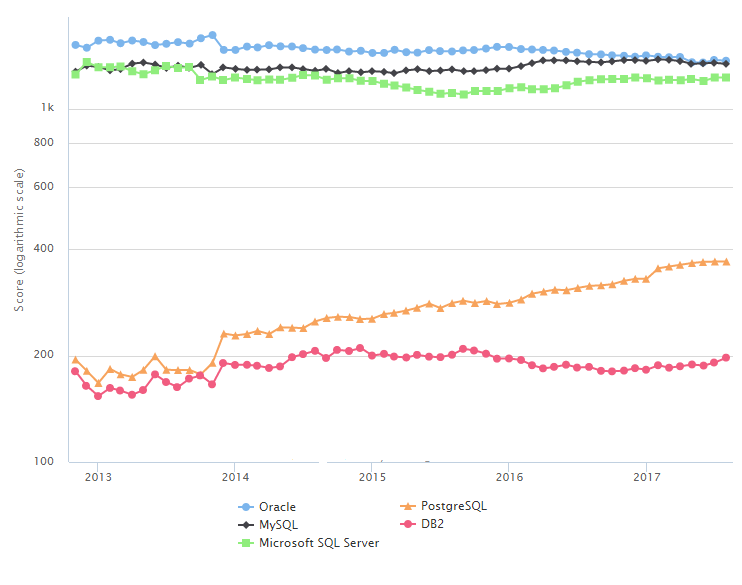
\includegraphics[width=\textwidth,height=6cm]{Images/db_engines_chart}
      \caption{Popularity of modern DBMSs}
      \label{fig: Popularity of modern DBMSs}
    \end{figure}

The Figure 2.1 illustrates the most popular DBMSs from 2013 to 2017 using a calculated score based on the Google Trend, number of mentions of DBMSs on the web and discussion of the systems in Stackoverflow and DBA Stack Exchange. It can be seen that the popularity of Oracle database, MySQL and Microsoft SQL Server remain constant over the years with a relatively high score. In addition, there is a stable rise for PostgreSQl in the last three years. Lastly, IBM DB2 popularity has decreased slightly in the last year. 



